\subsection{Leitungsschutz}
Beantworten Sie folgende Fragen:

\begin{enumerate}
    \item   \question{Wodurch kann in Verteilungsnetzen (EVU-Netz, Verbraucheranlage) Überstrom auftreten?} \\\\
            Durch den Anschluss einer Überlast oder durch einen Kurzschluss.
    \item   \question{Wie erfolgt der Schutz gegen Überstrom in Verbraucheranlagen?} \\\\
            Durch Einbau von Überstrom-Schutzorganen.
    \item   \question{Welche zwei Arten von Überstromschutzorganen kennen Sie?} \\\\
            Schmelzsicherungen und Leitungsschutzschalter.
\end{enumerate}

\subsubsection{Schmelzsicherungen}
Beantworten Sie die unten aufgelisteten Aufgabestellungen. Eine Begründung Ihrer Entscheidung ist essenziell.

\begin{enumerate}
    \item   \question{Welche Bauarten werden bei Schmelzsicherungen unterschieden?} \\\\
            Es wird zwischen Stöpselsicherungen und NH-Sicherungen (Niederspannungs-Hochleistung) unterschieden.

    \item   \question{Nennen Sie die wichtigsten Kenngrößen von Schmelzsicherungen} \\\\
            Bemessungsspannung, Bemessungsstrom, Bemessungsschaltvermögen und Betriebsklasse.

    \item   \question{Über welche Prüfströme wird die Auslösecharakteristik und Fertigungstoleranz einer Schmelzsicherung festgelegt? Wie sind diese Prüfströme definiert?} \\\\
            Durch den kleinen und großen Prüfstrom. Der kleine Prüfstrom bezeichnet den Strom, bei dem die Sicherung innerhalb der konventionellen Prüfdauer nicht schmelzen darf.
            Der große Prufström beschreibt jenen Strom, bei dem die Sicherung innerhalb einer konventionellen Prüfdauer ausschalten muss.

    \clearpage
    \item   \question{Erklären Sie Aufbau und Funktion einer Stöpselsicherung (+Skizze)} \\\\
            Folgende Abbildungen zeigen den Aufbau der Stöpselsicherung.
            \begin{figure}[!htp]
                \centering
                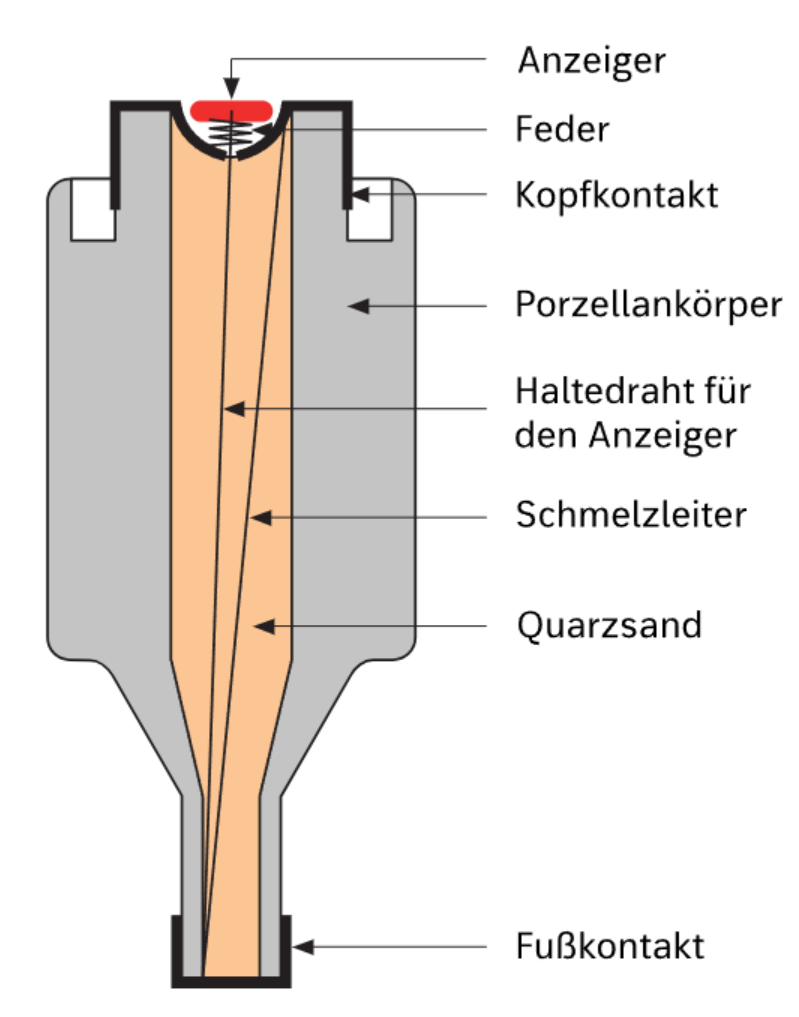
\includegraphics[scale = 0.3]{img/Stopsel_Aufbau.png}
            \end{figure}

            \begin{figure}[!htp]
                \centering
                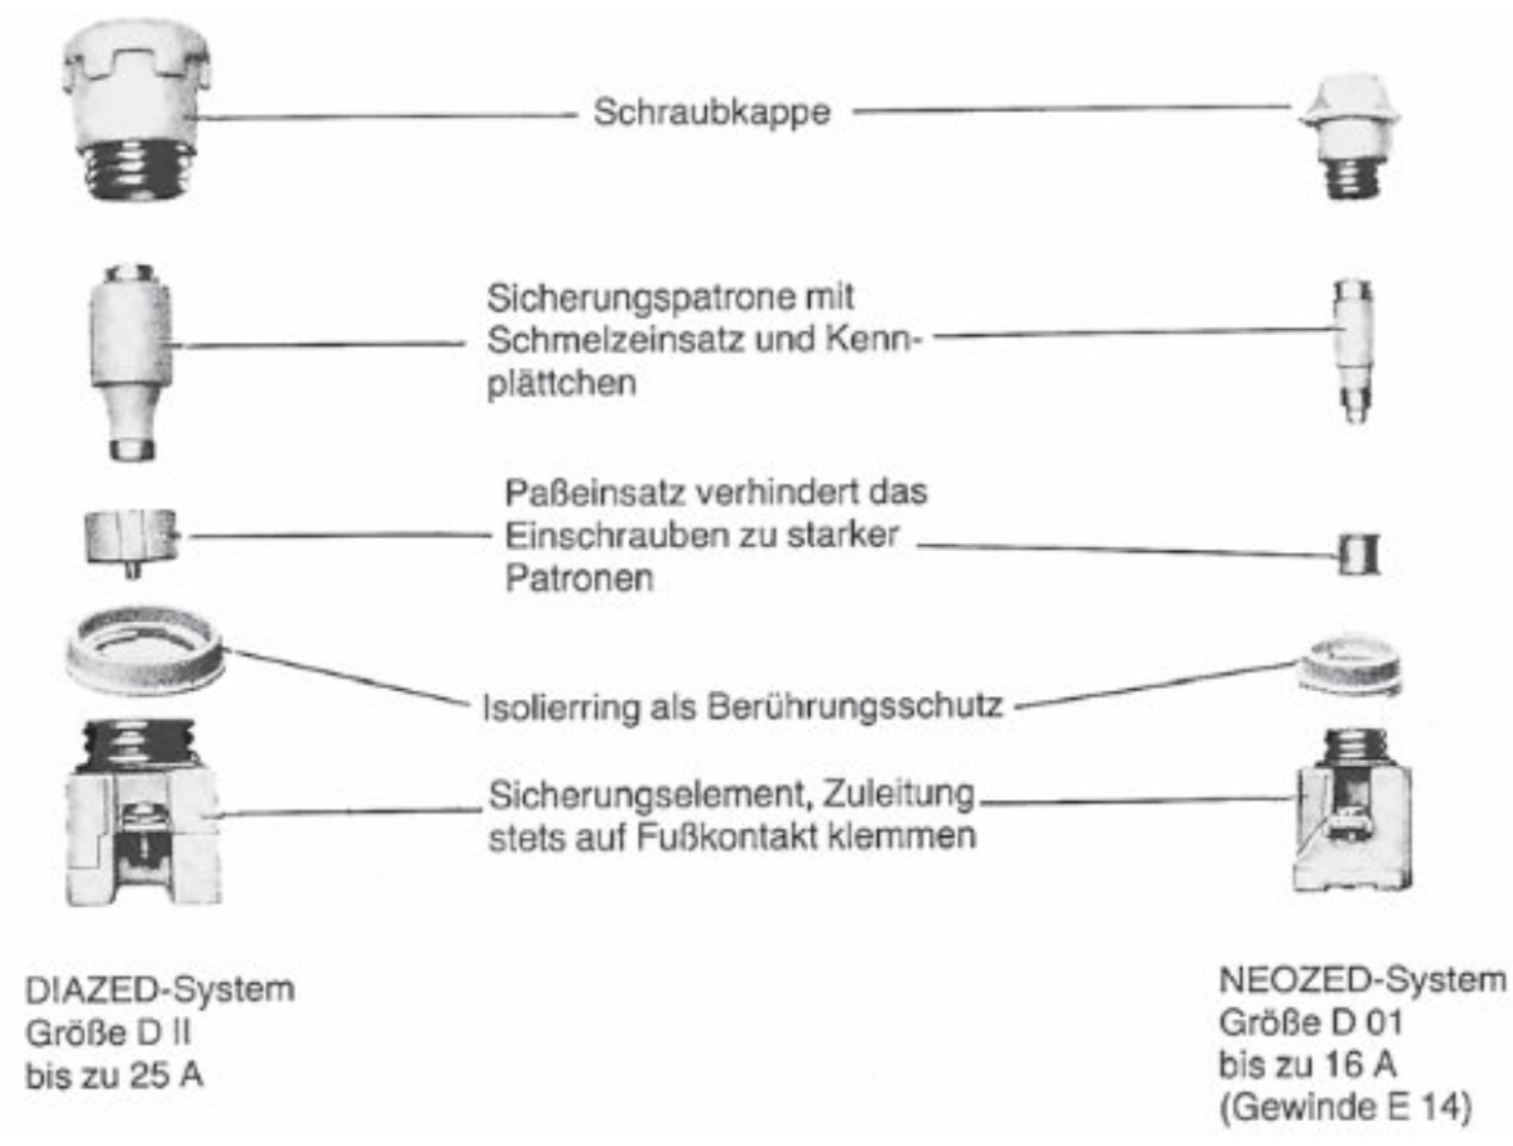
\includegraphics[width = 0.7\textwidth]{img/Stopsel_Aufbau_2.png}
            \end{figure}
            Die Sicherung stellt einen Überlastschutz und Kurzschlusschutz dar. Fließt ein zu hoher Strom, erhöht sich die Temperatur des Schmelzleiters, welcher 
            direttissima \footnote{Direttissima: Direkt; der kürzeste Weg.} schmilzt. Die Stöpselsicherungen werden heutzutage nur vereinzelt in Häusern verwendet.
            \clearpage

    \item   \question{Erklären Sie Aufbau und Funktion einer NH-Sicherung (+Skizze)}\\\\
            Folgende Abbildung zeigt den Aufbau der NH-Sicherung.
            \begin{figure}[!htp]
                \centering
                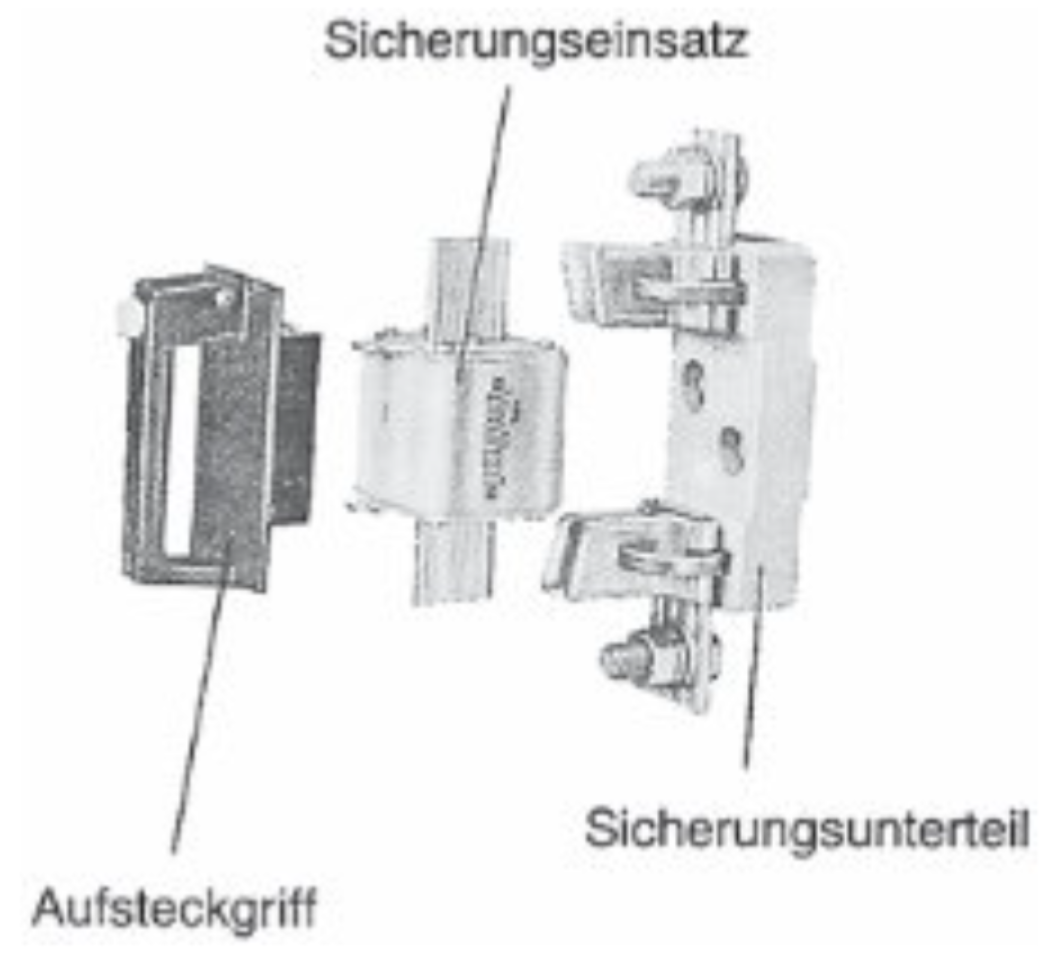
\includegraphics[scale = 0.3]{img/NH_Aufbau.png}
            \end{figure}
            \begin{figure}[!htp]
                \centering
                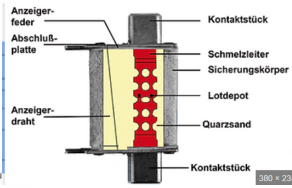
\includegraphics[scale = 0.3]{img/NH_Aufbau_real.PNG}
            \end{figure}

            Funktion: Abschaltung bei Überstrom oder Kurschluss. NH-Sicherungen sind für den Einbau in der Nähe von Transformatorstationen 
            und als Hausanschlusssicherung eingesetzt.

    \item   \question{Worüber gibt die Betriebsklasse einer Schmelzsicherung auskunft?} \\\\
            Die Betriebsklasse gibt über die Verwendbarkeit von Sicherungen und ihre Strom-Zeit-Kennlinie auskunft.

    \item   \question{Nennen Sie 3 Vorteile eines NH-Trenners gegenüber Stöpselsicherungen.} \\\\
            Ein NH-Lasttrenner bietet folgende Vorteile:
            \begin{itemize}
                \item Die massiveren Kontakte können größere Ströme führen
                \item Stromkreis wird dreipolig geschaltet
                \item Höheres Ausschaltvermögen
            \end{itemize}      

    \item   \question{Unter welchen Bedingungen werden Schmelzsicherungen gegenüber Leitungsschutzschaltern bevorzugt? (+Beispiele)}\\\\
            Wenn Selektivität benötigt wird. \textcolor{red}{Bsp.:?????}

    \clearpage


    \item   \question{Erklären Sie Aufbau und Funktion eines Leitungsschutzschalters. Wie erfolgt die Auslösung bei einem Leitungsschutzschalter.}\\\\

            \begin{figure}[!htp]
                \centering
                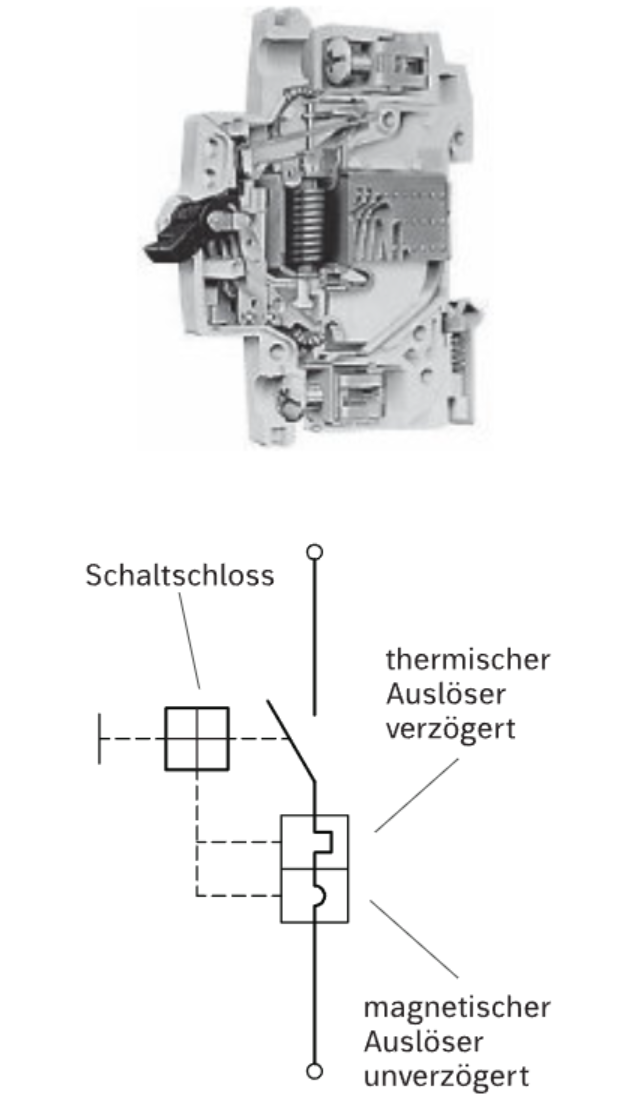
\includegraphics[width = 0.5\textwidth]{img/LSS_Aufbau.png}
            \end{figure}
            \begin{figure}[!htp]
                \centering
                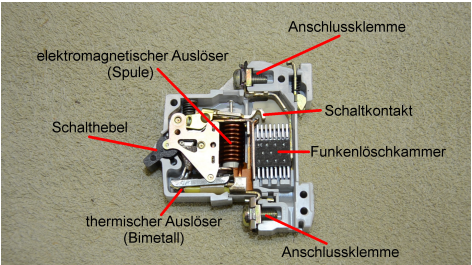
\includegraphics[width = 0.5\textwidth]{img/Leitungsschutzschalter.PNG}
            \end{figure}

            Ein Leitungsschutzschalter besitzt eine thermische (Überlastschutz) und magnetische (Kurzschlusschutz) Auslösung.

    \item   \question{Nennen Sie Vorteile von Leitungsschutzschaltern gegenüber Schmelzsicherungen.} \\\\
            Können wieder eingeschalten werden -> keine Ersatzsicherungen erforderlich -> kein Einsetzen einer falschen Sicherung möglich. Zudem lösen sie bei Kurzschlussen schneller durch. Leitungsschutzschalter lassen sich nicht überbrücken.
            Daraus folgt, dass Laien sich nicht mehr unter Gefahr setzen können. Sichere Bedienung. Kompakte Bauweise.  

    \clearpage

    \item   \question{Über welche Prüfströme  wird die Auslösecharakteristik und Fertigungstoleranz eines Leitungsschutzschalters festgelegt. Wie sind diese Prüfströme definiert?} \\\
            Es gibt folgende Auslösestrome:

            \begin{itemize}
                \item Nichtauslösestrom: jener Strom, bei dem der LSS nicht auslösen darf. 1,13-fache des Bemessungsstroms.
                \item Auslösestrom: jener Strom, bei dem der LSS innerhalb der festgelegten Prüfdauer ausschalten \textbf{muss}. 1,45-fache des Bemessungsstroms.
                \item Sofortauslösestrom: jener Strom, bei dem der LSS innerhalb $\SI{0.1}{s}$ abschaltet. Er hängt von der Type ab.
            \end{itemize}

    \item   \question{Wie unterscheiden sich Leitungsschutzschalter der Typen B, C und D in ihrer Auslösecharakteristik (+Skizze)?} \\\\
            Folgende Skizze beschreibt den Unterschied:

            \begin{figure}[!htp]
                \centering
                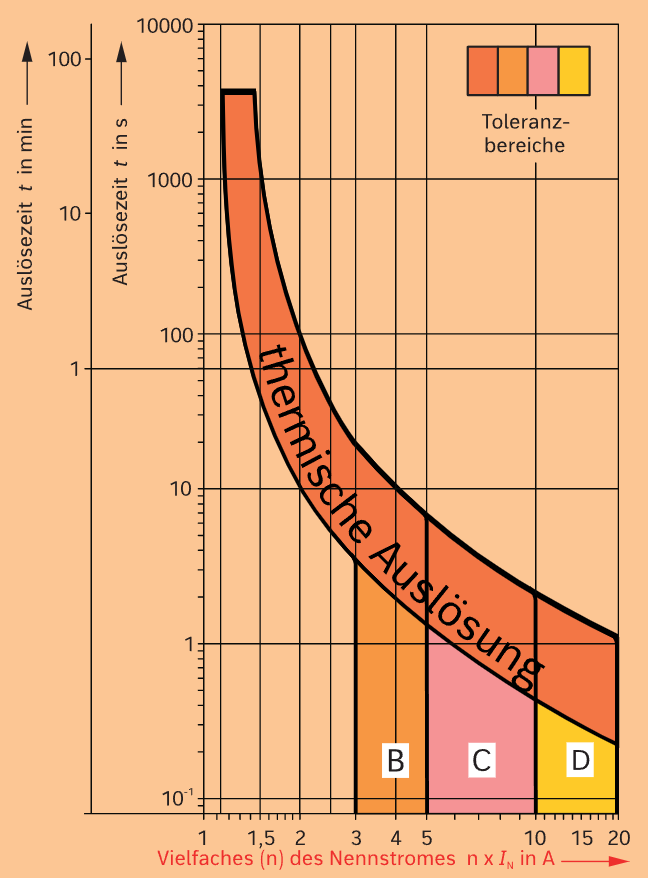
\includegraphics[width = 0.5\textwidth]{img/Auslosecharakteristik.png}
            \end{figure}

            Die thermische Auslösung ist äquivalent. Sie unterscheiden sich nur durch die magnetische Auslösung.
            Desto höher der Buchstabe, desto niedriger die Sensitivität über Spitzenströme.

    \clearpage

    \item   \question{Ein Winkelschleifer hat einen Nennstrom von 6A und nimmt beim Einschalten kurzzeitig den 8fachen Strom auf. Wird ein klagloser Betrieb möglich sein, wenn der Stromkreis mit einem 13A LS-Schalter vom Typ B abgesichert ist oder schlagen Sie einen anderen Leitungsschutzschalter vor? (+Begründung)} \\\\
            \textcolor{red}{TODO.} Ein Typ-C-Leitungsschutzschalter ist empfehlenswert.

    \item   \question{Worauf muss man bei der Verwendung von LS-Schaltern der Type D im genullten Netz achten?} \\\\
            Die Ausschaltbedingung muss erfüllt sein. Ist diese nicht erfüllt, so ist die Nullung nicht wirksam. Es besteht Lebensgefahr.

            Anhand folgender Formel lässt sich dies erklären:

            $$Z_S \le \frac{U_0}{I_A}$$

            $I_A$ ist bei Type D besonders groß. 

    \item   \question{Was versteht man unter der Energiebegrenzungsklasse eines Leitungsschutzschalters? Welche Auswirkung hat eine hohe Energiebegrenzungsklasse?} \\\\
            Die Energiebegrenzungsklasse eines LS-Schalters ist ein Maß für die Durchlassenergie, die ein Schalter benötigt, um den Stromkreis zu öffnen $\left(I^2\cdot t\right)$.
            Es gibt die Energiebegrenzungsklassen 1, 2 und 3. Je höher, desto niedriger ist die spezifische Durchlassenergie (bezogen auf den Bemessungsstrom), desto schneller schaltet der Schalter aus.         
\end{enumerate}

\subsubsection{Ausschaltstrom / Selektivität}
Lösen Sie folgende Aufgabenstellungen zum Thema Ausschaltstrom / Selektivität

\begin{enumerate}
    \item   \question{Wie ist der Ausschaltstrom von Überstromschutzorganen definiert?} \\\\
            Der Ausschaltstrom ist jener Strom, der fließen muss, damit ein Überstromschutzorgan im Fehlerfall so schnell ausschaltet, dass keine Gefahr durch indirektes Berühren entsteht.
            Dieser Strom wird als Vielfache des Nennstromes angegeben.

    \item   \question{Was versteht man unter Selektivität von Überstromschutzorgangen? Unter welcher Voraussetzung ist die Selektivität gegeben? Nennen Sie 2 einfache Regeln zur Selektivität.} \\\\
            Selektivität bedeutet, dass im Fehelrfallse nur jenes Überstromschutzorgan abschaltet, das sich unmittelbar vor der Fehlerstelle befindet, und alle anderen betriebsbereit bleiben.
            Durch die Selektivität wird die Betriebssicherheit einer Anlage erheblich verbessert.
            2 Regeln: \\
            - Schmelzsicherungen sind bei einem Nennstromverhältnis von 1 : 1,6 selektiv. \\
            - In der Reihe geschaltete Leitungsschutzschalter sind in der Regel bei Kurzschluss nicht selektiv (beide magnetischen Auslöser schalten ab).  
\end{enumerate}